% !TEX TS-program = pdflatex
% !TEX encoding = UTF-8 Unicode

% This is a simple template for a LaTeX document using the "article" class.
% See "book", "report", "letter" for other types of document.

\documentclass[11pt]{article} % use larger type; default would be 10pt

\usepackage[utf8]{inputenc} % set input encoding (not needed with XeLaTeX)

%%% PAGE DIMENSIONS
\usepackage{geometry} % to change the page dimensions
\geometry{a4paper} % or letterpaper (US) or a5paper or....

\usepackage{graphicx} % support the \includegraphics command and options

\usepackage{amssymb}
\usepackage{amsmath}
%%% PACKAGES
\usepackage{booktabs} % for much better looking tables
\usepackage{array} % for better arrays (eg matrices) in maths
\usepackage{paralist} % very flexible & customisable lists (eg. enumerate/itemize, etc.)
\usepackage{verbatim} % adds environment for commenting out blocks of text & for better verbatim
\usepackage{subfig} % make it possible to include more than one captioned figure/table in a single float
% These packages are all incorporated in the memoir class to one degree or another...

%%% HEADERS & FOOTERS
\usepackage{fancyhdr} % This should be set AFTER setting up the page geometry
\pagestyle{fancy} % options: empty , plain , fancy
\renewcommand{\headrulewidth}{0pt} % customise the layout...
\lhead{}\chead{}\rhead{}
\lfoot{}\cfoot{\thepage}\rfoot{}

%%% SECTION TITLE APPEARANCE
\usepackage{sectsty}
\allsectionsfont{\sffamily\mdseries\upshape} % (See the fntguide.pdf for font help)
% (This matches ConTeXt defaults)

%%% ToC (table of contents) APPEARANCE
\usepackage[nottoc,notlof,notlot]{tocbibind} % Put the bibliography in the ToC
\usepackage[titles,subfigure]{tocloft} % Alter the style of the Table of Contents
\renewcommand{\cftsecfont}{\rmfamily\mdseries\upshape}
\renewcommand{\cftsecpagefont}{\rmfamily\mdseries\upshape} % No bold!
\usepackage{tikz,forest}

\usepackage{amsmath}
\usepackage{graphicx}
\graphicspath{ {./pings/} }
\DeclareMathOperator*{\argmax}{arg\,max}
\DeclareMathOperator*{\argmin}{arg\,min}

\newcount\colveccount
\newcommand*\colvec[1]{
        \global\colveccount#1
        \begin{pmatrix}
        \colvecnext
}
\def\colvecnext#1{
        #1
        \global\advance\colveccount-1
        \ifnum\colveccount>0
                \\
                \expandafter\colvecnext
        \else
                \end{pmatrix}
        \fi
}
\usetikzlibrary{arrows.meta}

\forestset{
    .style={
        for tree={
            base=bottom,
            child anchor=north,
            align=center,
            s sep+=1cm,
    straight edge/.style={
        edge path={\noexpand\path[\forestoption{edge},thick,-{Latex}] 
        (!u.parent anchor) -- (.child anchor);}
    },
    if n children={0}
        {tier=word, draw, thick, rectangle}
        {draw, diamond, thick, aspect=2},
    if n=1{%
        edge path={\noexpand\path[\forestoption{edge},thick,-{Latex}] 
        (!u.parent anchor) -| (.child anchor) node[pos=.2, above] {Y};}
        }{
        edge path={\noexpand\path[\forestoption{edge},thick,-{Latex}] 
        (!u.parent anchor) -| (.child anchor) node[pos=.2, above] {N};}
        }
        }
    }
}

%%% END Article customizations

%%% The "real" document content comes below...

\title{Micro HW5}
\author{Michael B. Nattinger\footnote{I worked on this assignment with my study group: Alex von Hafften, Andrew Smith, Ryan Mather, and Tyler Welch. I have also discussed problem(s) with Emily Case, Sarah Bass, and Danny Edgel.}}

%\date{} % Activate to display a given date or no date (if empty),
         % otherwise the current date is printed 

\begin{document}
\maketitle

\section{Question 1}
Rowena will take the larger of the two pieces of cake. Therefore, Colin will always be stuck with the smaller of the two pieces of cake. Colin, therefore, will maximize his utility by making the smallest piece of cake as large as possible. The largest that the smallest piece of cake can be is half the size of the cake, lest it becomes the largest piece of cake. Therefore, Colin will split the cake exactly in half, and Rowena will take either of the two evenly sized slices.

\section{Question 2}
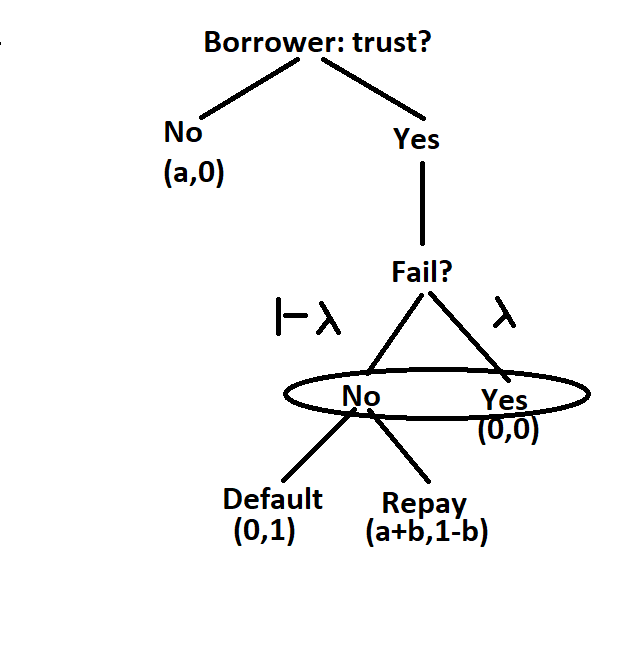
\includegraphics{extform}

From the above game tree, we can deduce the subgame perfect equilibrium by backwards induction. If the project occurs and does not fail, then the lender does not have any reason to repay their investments. They are strictly better off by not repaying. So, they will not repay. Therefore, when the investor looks at the game tree in front of them, they see an expected utility from investing of 0, and an expected utility from not investing of a. They will choose not to invest. So, the subgame perfect equilibrium is for the investor to not invest.

\section{Question 3}
\subsection{Part A}
For $n=1$, once the coin is flipped then the offer should be accepted, as their payoff for accepting the offer is (weakly) greater than their payoff for rejecting the offer (0). Therefore, whomever wins the coin toss knows that their offer will be accepted, so they should offer 0 to the other person and 1 for themselves. Each person thus has a probability 1/2 to win the coin flip, and a payoff of 1 if they win the coin flip and 0 if they lose, so their expected utility is $1/2$.
\subsection{Part B}
For $n=2$, if the offer is declined in the first round then the expected payoff of each person is $\delta (1/2)$. Therefore, in the first round, the person that loses the coin toss will accept any offer (weakly) greater than $\delta (1/2)$. The person who wins the coin toss can gain $1-\delta(1/2)>\delta(1/2)$ if they offer $\delta(1/2)$ to the second person so they will offer that amount and the second person will accept. Their expected utility, therefore, is $(1/2)(1-\delta(1/2)) + (1/2)(\delta(1/2)) = 1/2$.
\subsection{Part C}
For $n\geq 3$, we work backwards from the last period. Their expected utility of entering into that last period is $\delta^{n-1}(1/2)$. In the period prior, the discounted expected utility of entering into that last period is the bid that would be accepted, so $\delta^{n-2}(1/2)$ is the lowest amount that the person who lost the coin toss would accept. In each period proceeding backwards, the accepted bids proceeds in the same fashion, with one fewer exponent of the geometric decay factor at a time, until the first period. In this first period, following the trend, the discounted expected utility of entering into that last period is $\delta(1/2)$, and so this is the lowest amount that the individual that loses the coin toss will accept, and the payoffs thus are the same as iin Part B, $1-\delta(1/2)$ for the winner of the coin toss and $\delta(1/2)$ for the loser.

\section{Question 4}
The two coffee shops will choose locations to maximize revenue, given the location of the other firm and their pricing functions. We can work backwards to find the subgame perfect nash equilibrium.

Given the coffee shop locations and the price of the competitor, the return of setting a price is the following:

\begin{align*}
\pi (p_i|p_{-i},x_i,x_{-i}) &= p_i \int_{0}^{1}1\{c(w-x_i)^2+p_i<c(w-x_{-i})^2+p_{-i}\}dw
\end{align*}
The coffee shops will choose prices to maximize profits. We will solve by taking first order conditions:

\begin{align*}
\max_{p_i} \pi (p_i|p_{-i},x_i,x_{-i}) &= \max_{p_i} p_i \int_{0}^{1}1\{c(w-x_i)^2+p_i<c(w-x_{-i})^2+p_{-i}\}dw\\
0&=\int_{0}^{1}1\{c(w-x_i)^2+p_i<c(w-x_{-i})^2+p_{-i}\}dw +p_i\int_{0}^{1}1\{c(w-x_i)^2+p_i=c(w-x_{-i})^2+p_{-i}\}dw
\end{align*}
\end{document}
